\documentclass[12pt, letterpaper]{article}
\usepackage[utf8]{inputenc}
\usepackage[czech]{babel}
\usepackage{indentfirst}
\usepackage{listings}
\usepackage{caption}
\usepackage{float}
\usepackage{graphicx}
\usepackage{hyperref}
\usepackage{textcomp}
\usepackage{array}
%%%
%%%
\begin{document}
%%%
%%% TITLE PAGE
%%%
\begin{titlepage}
\centerline{
\includegraphics[width=10cm]{img/logo}}
\begin{center}
\vspace{30px}
{\huge
\textbf{Vyhledávání informací}\\
\textbf{Komplexní IR systém}\\
\vspace{1cm}
}
{\large
\textbf{KIV/IR}\\
\vspace{1cm}
}
\vspace{1cm}
{\large
Pavel Třeštík\\
}
{\normalsize
A22N0137P
}
\end{center}
\vspace{\fill}
\hfill
\begin{minipage}[t]{7cm}
\flushright
\today
\end{minipage}
\end{titlepage}
%%%
%%% TEXT START
%%%
\section{Úvod a analýza}
Cílem práce je implementovat systém na vyhledávání informací. Komplexní v této práci znamená to, že
program umožňuje předzpracovat dokumenty, za indexovat množinu dokumentů a nad nimi implementovat alespoň 2 vyhledávací
modely. Zdroj dat byl
zvolen na prvním cvičení tohoto předmětu. Tato práce bere data získaná z \url{https://en.wikipedia.org}. Crawler
(nebo česky pavouk) získávající data z webu není součástí této práce, ale byl odevzdán na prvním cvičení. Je také
poskytnuto rozhraní pro semestrální práci, které by se mělo dodržet.

První částí práce je preprocessing. Je požadována jak \texttt{tokenizace}, tak \texttt{stemming} či \texttt{lemming}.
Tokenizace je přímočará a jedná se pouze o rozdělení textu. Další zpracování slouží k převedení slov
do základní formy, aby se dala snáze indexovat stejná slova, která se mohou lišit například pouze rodovou koncovkou.

Druhá část je samotné indexování. Zadání specifikuje, že se musí jednat o \texttt{invertovaný index}, tedy index,
ve kterým se ukládá seznam ID dokumentů pro každý \texttt{term} (zpracované slovo) jako klíč. Zadání požaduje pouze
\texttt{in-memory} index, ale za bonusové body je možné implementovat i ukládání indexu do souboru.

Třetí část je vyhledávání dotazů nad vytvořeným indexem. Zadání požaduje 2 typy dotazování a těmi jsou
\texttt{kosinová podobnost} a \texttt{logické vyhledávání}. Vrácené výsledky jsou řazené podle relevance, která
musí nějak vycházet z použitého typu dotazování.

Poslední částí je vhodně popsat implementaci a uživatelskou příručku v dokumentaci práce.
%
\section{Uživatelská příručka}
Výsledkem práce je CLI (Command Line Interface) aplikace. Tedy uživatel program ovládá z příkazové řádky.
Ovládání aplikace je realizováno pomocí příkazů (dále command) a často \uv{podpříkazů} (dále subcommand) s parametry.
Asi není potřeba podrobně popisovat úplně všechny příkazy, ale jen ty nejdůležitější a nejrelevantnější. Všechny
dostupné příkazy, jejich způsob použití a vysvětlení jejich funkčnosti může být viděn na Obrázku \ref{fig:help}.

Každý command a subcommand má dlouhou a krátkou formu. Na příklad příkaz \textbf{print page 8} může by zkrácen na
\textbf{p p 8}. Příslušné zkratky jsou také na Obrázku \ref{fig:help}.

Program umožňuje uživateli vytvořit více indexů bez nutnosti restartu programu. Je také možné nastavit způsob
indexování dat pro každý index, před jeho vytvořením. Všechny příkazy a některé dotazy jsou ale vykonávány pouze
nad zrovna zvoleným indexem. Zvolený index je samozřejmě možné změnit příslušným příkazem.

\begin{figure}[H]
    \centering
    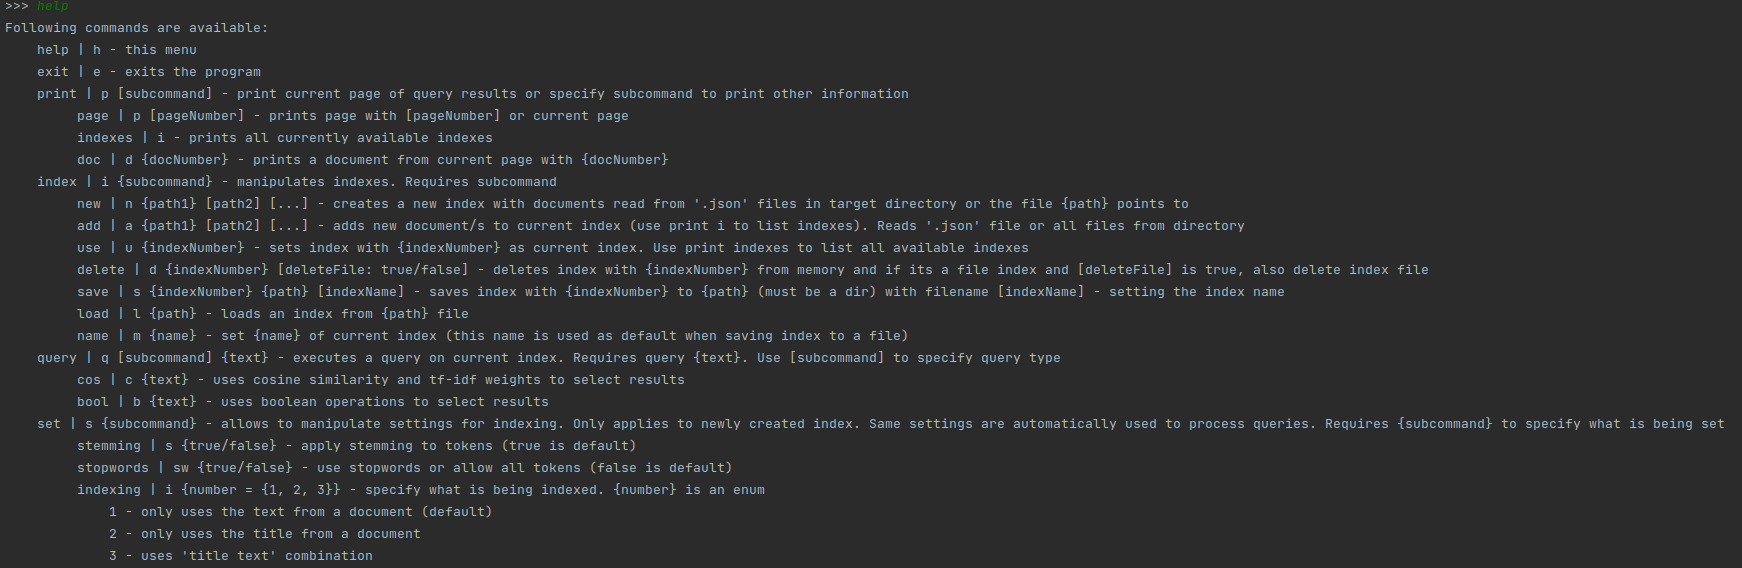
\includegraphics[width=\linewidth]{img/help}
    \caption{Výpis příkazu help}
    \label{fig:help}
\end{figure}
%
\subsection{Command: print $|$ p}
Command print je možné použít bez parametrů, ale v tomto případě se pak jedná o zkratku pro subcommand \textbf{page},
který vypíše poslední zobrazenou stránku. Pro zobrazení více specifických informací je třeba použít příslušný
subcommand. Těmi jsou \textbf{page}, \textbf{indexes}, \textbf{doc}.
%
\subsubsection{Subcommand: page $|$ p}
Jako parametr je nutné poskytnout číslo stránky. Při poskytnutí validního čísla stránky bude tato stránka vypsána.
Obsahem stránky je seznam výsledků (resp. podmnožiny výsledků), které byly získány posledním dotazem. Jednotlivé
výsledky jsou číslovány. Pro významné použití příkazu proto musí být nejdříve zadán nějaký dotaz. Při zadání
dotazu je automaticky vypsána první stránka výsledků.

\begin{figure}[H]
    \centering
    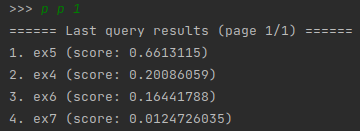
\includegraphics[width=\linewidth]{img/p_p}
    \caption{Příkaz 'print page 1' nad dotazem ze cvičení (q tropical fish sea)}
    \label{fig:p_p}
\end{figure}
%
\subsubsection{Subcommand: indexes $|$ i}
Tento subcommand nebere žádné parametry - pokud jsou nějaké poskytnuty, tak jsou ignorovány. Subcommand vypíše
očíslovaný seznam všech indexů co jsou zrovna v paměti a tedy mohou být použity. Index, který je zrovna vybrán a nad
kterým se provádí dotazy je označen jako např. \texttt{1 (current). Index...} - tedy obsahuje \textbf{current}.
%
\subsubsection{Subcommand: doc $|$ d}
Tento subcommand požaduje jeden parametr, kterým je číslo dokumentu. Subcommand vypíše název a obsah zvoleného
dokumentu. Číslo dokumentu odpovídá číslu vypsanému na stránce příkazem \textbf{print page X}.
%
%
\subsection{Command: index $|$ i}
Command index vyžaduje subcommand. Dostupné subcommandy jsou: \textbf{new}, \textbf{add}, \textbf{use}, \textbf{delete},
\textbf{save}, \textbf{load}, \textbf{name}.
%
\subsubsection{Subcommand: new $|$ n, add $|$ a}
Subcommand \textbf{new} vytváří nový index. Subcommand \textbf{new} přidává dokumenty do zrovna \texttt{zvoleného}
indexu. Oba dva tyto subcommandy přijímají stejné parametry, kterými jsou cesty do adresářů nebo souborů, ze kterých
se čtou dokumenty. Alespoň jedna cesta je požadována, ale je možné zadat libovolný počet cest, ze kterých se dokumenty
načítají.

Dokumenty jsou načítány z JSON souborů. Cesta předána subcommandu může být adresář, v tom případě jsou přečteny všechny
soubory, které mají příponu \texttt{.json}. Nebo předaná cesta vede na jeden konkrétní \texttt{.json} soubor, který
je načten samostatně.

Při načítaní dokumentů je nutné, aby měl každý dokument unikátní ID. Pokud dokument má duplicitní ID, a dokument s tímto
ID je již načten, tak nově čtený dokument je přeskočen. ID dokumentů jsou řetězce a v datech pro tuto práci jsou jako ID
použity části URL odkazů na Wikipedia článek.

Načítaný dokument musí mít následující strukturu:
\begin{lstlisting}[caption=Struktura JSON souboru s indexovatelnými dokumenty, captionpos=b]
{
  "docId1": {
    "title": "example 1"
    "timestampCrawled": "2023-05-06T16:23:39.686+02:00"
    "content: "long text 1"
  },
  "docId2": {
    "title": "example 2"
    "timestampCrawled": "2023-05-06T16:24:39.686+02:00"
    "content: "long text 2"
  },
  ...
}
\end{lstlisting}
%
\subsubsection{Subcommand: save $|$ s}
Subcommand \textbf{save} uloží index vybrán jedním z parametrů do souboru. Jsou požadovány 2 parametry a 1 dobrovolný.
Požadované parametry jsou: číslo indexu, který bude uložen a adresářová cesta, kam bude index uložen. Dobrovolným
parametrem je řetězec, který je aplikován jako jméno indexu.

Druhý parametr musí být adresář. Index je do tohoto adresáře uložen buď jako jméno indexu nebo pod časovou známkou
v momentu uložení.
%
\subsubsection{Subcommand: load $|$ l}
Subcommand \textbf{load} načte index ze souboru, který je načten z parametru. Požadován je jeden parametr, kterým je
cesta k indexovému souboru. Index je po načtení nastaven jako \texttt{zvolený}. Při načítání indexu jsou do cache
načteny i dokumenty indexu, protože není implementovaný \uv{lazy loading}.
%
\subsubsection{Subcommand: delete $|$ d}
Subcommand \textbf{delete} smaže index, který je vybrán parametrem. Je požadován 1 parametr, kterým je číslo indexu,
který má být smazán. Navíc je možné předat i 1 nepovinný parametr, kterým je logická hodnota (true/ false), která
určí, zda-li má být smazán i soubor indexu. Za předpokladu, že mazaný index je uložen i v souboru. To znamená, že
je možné smazat index pouze z paměti, ale stále zachovat uložený soubor. Index není automaticky ukládán při smazání,
takže pokud  je index modifikován a uživatel si ho přeje smazat pouze z paměti, tak je třeba ho nejprve ručně uložit.
%
%
\subsection{Command: query $|$ q}
Command \textbf{query} nevyžaduje specifikaci subcommand. Pokud subcommand není specifikovaný, tak se automaticky předpokládá
subcommand \textbf{cos}. Dostupnými subcommandy jsou: \textbf{cos}, \textbf{bool}.
%
\subsubsection{Subcommand: cos $|$ c}
Subcommand \textbf{cos} vyžaduje text jako parametr. Text je poté zpracován jako dotaz. Dotaz je vyhodnocen
kosinovou podobností využitím TF-IDF vah. Dotazem je tedy pouze text a každé slovo, které se v indexu nachází
přispívá k relevanci výsledku.

\begin{figure}[H]
    \centering
    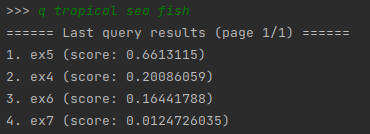
\includegraphics[width=\linewidth]{img/q_practice}
    \caption{Cosine similarity dotaz: tropical fish sea)}
    \label{fig:q_practice}
\end{figure}
%
\subsubsection{Subcommand: bool $|$ b}
Subcommand \textbf{bool} vyžaduje text jako parametr. Text je poté zpracován jako logický výraz. V dotazu
je možné použít operátory \texttt{AND}, \texttt{OR}, \texttt{NOT}. Pokud mezi slovy není specifikován operátor, tak
se automaticky předpokládá \texttt{AND}. Logické operátory není možné řetězit - tedy pokud bude použit například
dotaz \texttt{slovo1 AND OR NOT slovo2}, tak se dotaz zpracuje jako \texttt{slovo1 NOT slovo2}, protože se dotaz
vykonává z leva a platí pouze poslední operátor.

Je také možné použít závorky pro určení priority části dotazu. Zde ovšem uživatel může narazit na chybu implementace,
protože navzdory prioritě jsou výsledky částí dotazů spojovány v určitém pořadí a to může být chybné o proti prioritě.
Tato chyba je následkem chybné implementace. Na obrázku \ref{fig:bool_correct} lze vidět správně vykonaný dotaz a
očekávané výsledky. Na obrázku \ref{fig:bool_wrong} je velmi podobný dotaz, který by měl dávat stejné výsledky,
ale kvůli chybě ve spojování priorit vrací špatné výsledky.

\begin{figure}[H]
    \centering
    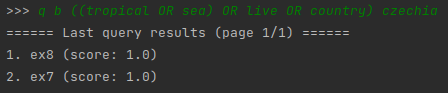
\includegraphics[width=\linewidth]{img/bool_correct}
    \caption{Příklad booleovského dotazu, kde jsou priority správně}
    \label{fig:bool_correct}
\end{figure}

\begin{figure}[H]
    \centering
    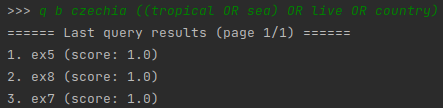
\includegraphics[width=\linewidth]{img/bool_wrong}
    \caption{Příklad booleovského dotazu, kde jsou priority špatně}
    \label{fig:bool_wrong}
\end{figure}
%
\subsection{Command: set $|$ s}
Command \textbf{set} vyžaduje subcommand. Subcommandy jsou: \textbf{stemming}, \textbf{stopwords} a \textbf{indexing}.
S využitím subcommandů je tímto možné nastavit některé parametry indexování dokumentů pro nově vytvořený index.
Tyto parametry jsou také aplikovány při zpracování dotazů.
%
\subsubsection{Subcommand: indexing $|$ i}
Subcommand \textbf{indexing} vyžaduje jeden číselný parametr. Toto číslo musí být v rozmezí $<1,3>$ a nastavuje
následující vlastnost:
\begin{itemize}
    \item 1 - indexován je pouze text dokumentu (content)
    \item 2 - indexován je pouze název dokumentu (title)
    \item 3 - indexován je název spojen s textem dokumentu
\end{itemize}
%
%
%
\section{Implementace}
V této části jsou popsány implementace některých částí práce a případné problémy s jejich řešením.
%
\subsection{Preprocessing}
Preprocessing (nebo česky předzpracování) je v programu použit na několika místech. Těmi je indexování a parsování
dotazů. Aby bylo zajištěno, že dotaz je zpracován stejným způsobem jako indexovaná data, tak je preprocessing volán
z třídy \textbf{Preprocessor}, která je singleton.
%
\subsubsection{Tokenizace}
Tokenizace v této práci má pokročilejší implementaci. To znamená, že dělení textu na slova není realizováno pouze
dělením bílými znaky, ale porovnáním proti regexu, který umožňuje vyextrahovat url, cifry, datumy, apod. Tokenizer
je navíc rozšířen o možnost vyhazování stop slov (stopwords). Protože data pochází z anglické wikipedie, tak
s prací je poskytnut použitý seznam anglických stopwords.

Tokenizace je implementována ve třídě \textbf{AdvancedTokenizer} a implementuje poskytnuté rozhraní \textbf{Tokenizer}.
Vstupní data jsou vždy tokenizována, ale je možné vybrat zda-li mají být použita stopwords - toto nastavení se nachází
ve třídě \textbf{IndexSettings}.
%
\subsubsection{Stemming}
Pro další zpracování dat byl vybrán stemming pro jeho jednoduchost aplikování na slovo. Nevýhodou stemmingu je, že
nekontroluje sémantický význam slova, takže mohou vznikat nesmyslné výsledky, které jsou poté v indexu. Další nevýhodou
je, že stemming/ lemming je specifický dle jazyka, což je relativně velkou nevýhodou v této práci, protože data pochází
z Wikipedie. Ačkoliv jsou data získána z anglické verze Wikipedie, tak se velmi často objevují jednotlivá slova či názvy
v jiných jazycích, než je angličtina.

Byl použit anglický stemmer třetí strany. Tento stemmer se nachází v balíčku
\textbf{preprocessing.RovoMe.EnglishStemmer} a je možné ho získat z GitHubu
\url{https://github.com/RovoMe/PorterStemmer}. Stemmer byl rozšířen pouze o implementaci poskytnutého rozhraní
\textbf{Stemmer}, což je požadováno zadáním. Zda-li se má stemming aplikovat, je možné nastavit v
\textbf{IndexSettings}.
%
%
\subsection{Index}
Zadání požaduje, aby byl index implementován jako invertovaný index. Indexem tedy je mapa termů (zpracované slovo), kde
klíčem je term a hodnotou klíče je seznam dokumentů, ve kterých se tento term nachází. V základní podobě indexu jsou
v seznamu ukládána pouze ID dokumentů, ale v této práci jsou ukládány objekty \textbf{IndexEntry}, což je pomocná třída,
která obsahuje referenci na dokument (instance pomocné třídy \textbf{DocumentRef}), frekvenci výskytů slova v dokumentu
a TF-IDF váhu, kterou term má v daném dokumentu. Tyto údaje jsou použity pro vyhledávání kosinovou podobností a
frekvence výskytu je použita k určení relevance dokumentu v booleovských dotazech. \textbf{DocumentRef} obsahuje
pouze ID dokumentu a celkovou sumu čtverců dokumentu, která je potom odmocněna (normována) v kosinové podobnosti.

Index také obsahuje některé dodatečné informace, kterými jsou:
\begin{itemize}
    \item mapování ID dokumentů na reference dokumentů - aby se předešlo duplikaci referencí na stejný dokument a
        snazší přístup
    \item absolutní cesty k dokumentům - aby bylo možné načíst indexované dokumenty při načítání indexu ze souboru
    \item počet dokumentů v indexu
    \item nastavení indexu - zda-li aplikovat stopwords, stemming a způsob indexování textu
\end{itemize}
%
%
\subsection{Vyhledávání}
Implementovány jsou 2 způsoby vyhledávání. Těmi jsou \textbf{cosine similarity} a \textbf{boolean search}.
%
\subsubsection{Cosine similarity}
Cosine similarity (česky kosinová podobnost) je způsob porovnávání podobnosti dokumentů využitím TF-IDF vah. Tato
podobnost je počítána vzorcem viz Obrázek \ref{fig:cos_similarity} (obr. z wiki). V této práci je implementována ve
třídě \textbf{CosineSimilarity}.

\begin{figure}[H]
    \centering
    
\includegraphics[width=\linewidth]{img/cos_formula}
    \caption{Vzorec kosinové podobnosti}
    \label{fig:cos_similarity}
\end{figure}

Pro každý term dotazy je získán příslušný seznam IndexEntry objektů. Problémem je, že z indexu dostaneme pouze seznam
dokumentů pro term. My ale potřebujeme spočítat váhu pro každý relevantní dokument, ne pro term. Proto je třeba
seskupit relevantní dokumenty podle jejich referencí (\textbf{DocumentRef}, teoreticky by stačilo jako ID, ale v
indexu jsou použity tyto objekty). Zároveň ale potřebujeme znát, které termy jsou v dokumentu relevantní a tím nám
vznikne konstrukce mapa map seznamů. Nejedná se o nejhezčí
konstrukci, ale je pak snadné tímto spočítat kosinovou podobnost.

Ta je spočtena dle vzorce \ref{fig:cos_similarity} . Zde ušetříme čas procesoru tím, že již máme spočteny sumy vah
čtverců pro každý dokument. To je spočítáno při indexaci. Také nám stačí spočítat sumu čtverců dotazu pouze jedinkrát
pro dotaz. Pro každý relevantní dokument tedy musíme spočítat jen sumu násobků v čitateli.

Nakonec stačí vytvořit seznam výsledků, který je seřazen podle spočtené podobnosti.
%
\subsubsection{Boolean search}
V boolean search/ query (česky logický výraz) je pro každý term získán seznam dokumentů a nad seznamy dokumentů se
poté provádí logické akce \texttt{AND}, \texttt{OR} a \texttt{NOT}. Výraz je možné rozdělit na menší části, které
jsou vykonávány prioritně pomocí závorek. Implementace zpracování těchto dotazů je v této práci implementována
manuálně - tedy bez použití knihoven třetích stran (např. Lucene).

Dotaz je vyhodnocován zleva. Prozatím je ignorována priorita závorkami. Protože výraz je vyhodnocován z leva, tak jednotlivé
operace fungují následovně. Výsledek prvního termu je vložen do konečného seznamu výsledků dotazu. Poté jsou čteny
další tokeny. Pokud je token logický operátor, tak se pouze nastaví proměnná operátoru a čte se další token. Pokud
je další token term, tak se získá jeho seznam seznam výsledků. Poté jsou seznamy spojeny operací, která je uložena
v  proměnné operátoru. Máme tedy 2 seznamy. \uv{První} (levý, první term) a \uv{druhý} (pravý, druhý term).
Operátory fungují následovně:
\begin{itemize}
    \item AND - výsledkem AND operace je pouze první seznam, ze kterého jsou odstraněny záznamy, které nejsou
        v obou seznamech. Záznamy, které jsou v obou seznamech jsou sloučené dohromady.
    \item NOT - výsledkem NOT operace je pouze odstranění všech záznamů druhého seznamu z prvního. Jeden z důvodů proč
        se vykonává pouze poslední logický operátor (pokud jich je zřetězeno více za sebou) je to, aby nevznikl operátor
        \textbf{OR NOT}, který by byl velice náročný a pravděpodobně by obsahoval velice velkou část celého indexu.
    \item OR - výsledkem OR operace je první seznam sloučen s druhým. Klíče, které existují pouze v druhém seznamu
        jsou přidány do prvního a hodnoty klíčů existující i v prvním seznamu jsou sloučeny.
\end{itemize}

Nyní je přidáno zpracování závorek. Závorky v podstatě dělí dotaz na více malých dotazů a výsledky těchto dotazů by mělo
být možné sloučit stejným způsobem jako seznamy pro term. V implementaci ale vzniká problém ten, že výsledkem
termu je seznam záznamů v indexu. Výsledkem dotazu či jeho části ale je mapa, kde klíčem je dokument ID a hodnotou je
seznam záznamů v indexu pro tento dokument. Ačkoliv se tedy aplikují stejné logické operátory a provádí se stejná
operace, tak je ale třeba oddělené implementace (nejde tedy použít stejnou metodu).

Celkově pro vyhodnocování logického výrazu by bylo možné použít strom. V této části už je ale dotaz zpracováván z leva
a ne stromově. Je tedy nutné využít jiný způsob vyhodnocení. Dotaz či jeho \uv{pod-dotaz} může mít technicky pouze formu
\texttt{prefix (infix) suffix}. Například rekurzí je poměrně snadné vyhodnotit prefix a infix a ty spojit do sebe.
Celkově pak ale vzniká problém, jak a kam se vlastně připojí suffix - jak se dá zjistit, kde suffix začíná a končí?

Tento problém byl nakonec řešen tak, že jsou nejdříve připraveny \uv{pod-dotazy} dle závorek a těm je přidělena
priorita podle zanoření - priorita = hloubka zanoření. Ty jsou poté zpracovány a podle priority spojovány.
Tímto řešením ovšem vznikly další nepředvídané problémy. Například dotaz \texttt{(sub query 1) OR (sub query 2)} je
těžké spojit, protože ačkoliv je správně rozdělen do 3 \uv{pod-dotazů}, tak 2 \uv{pod-dotaz} je pouze operátor OR,
s čímž nebylo počítáno a mergování bylo prováděno vždy použitím operátoru na konci \uv{pod-dotazu} (výchozí AND).
Tento problém, byl vyřešen tím, že byla zavedena pomocná privátní třída \textbf{ProcessedClause}, která obsahuje
operátor spojení na začátku i na konci \uv{pod-dotazu} a lze tedy určit, jestli je \uv{pod-dotaz} pouze spojem mezi
2mi druhými \uv{pod-dotazy}.

Před odevzdáním ale byl objeven nový závažný problém, který by bylo velice složité řešit s využitím tohoto způsobu
zpracování priorit. Tímto problémem je, že do zásobníku se odkládají mezivýsledky, dokud se nedorazí do \uv{pod-dotazu}
s nejvyšší prioritou. V moment kdy se do tohoto \uv{pod-dotazu} dorazí, tak se všechny výsledky ze zásobníku slučují do
jednoho až do vyprázdnění zásobníku. To je ovšem problém, protože se takhle nespojí případné suffixy dotazu. V odevzdané
verzi práce je tento problém bohužel stále přítomný a nelze správně vykonat například dotaz \ref{fig:bool_wrong}.
%
%
\section{Výsledky}
Práce implementuje funkčnosti viz Tabulka \ref{table:implemented}.

\begin{table}[H]
    \begin{center}
        \begin{tabular}{ | m{0.5\textwidth} | m{0.5\textwidth} | }
            \hline
            Tokenizace                                      & Booleovský model (AND, OR, NOT) \\
            \hline
            Preprocessing - stopslova                       & Priorita závorkami \\
            \hline
            Preprocessing - stemmer                         & Dokumentace\\
            \hline
            In-memory invertovaný index                     & File-based index \\
            \hline
            TF-IDF model                                    & Pozdější doindexování dat \\
            \hline
            Kosinová podobnost                              & Vlastní implementace vyhledávání dotazů \\
            \hline
            Vyhledávání vrací top X výsledků dle relevance  & \\
            \hline
        \end{tabular}
        \caption{Implementované funkčnosti}
        \label{table:implemented}
    \end{center}
\end{table}

Výsledky evaluace lze dělit na podle kosinové podobnosti a booleovského vyhledávání. Kosinová podobnost s využitím
TF-IDF vah funguje zcela správně. Výsledky byly ověřeny indexací dokumentů ze cvičení a použitím shodných dotazů
jako na cvičení. Příklad jednoho takovéhoto dotazu můžeme vidět na Obrázku \ref{fig:q_practice}.

Booleovské vyhledávání nebylo úplně proti čemu ověřit, ale na druhou stranu dává logický smysl. Tedy pokud nad
daty ze cvičení (Obrázek \ref{fig:data}) pustíme například dotaz \textbf{q b tropical OR sea}, tak očekáváme 3
dokumenty (Obrázek \ref{fig:bool_one}). V datech můžeme snadno dohledat, které dokumenty obsahují slovo
\texttt{tropical} nebo \texttt{sea}. Několika podobnými dotazy můžeme snadno ověřit funkčnost booleovského vyhledávání.

Pokud ovšem začneme používat závorky pro určení priority tak můžeme narazit na implementační chybu, kdy se dotaz
nevyhodnotí správně. Toto můžeme vidět na Obrázcích \ref{fig:bool_correct} a \ref{fig:bool_wrong}. Bohužel tato
chyba bylo objevena až těsně před odevzdáním a nebylo možné ji opravit.

\begin{figure}[H]
    \centering
    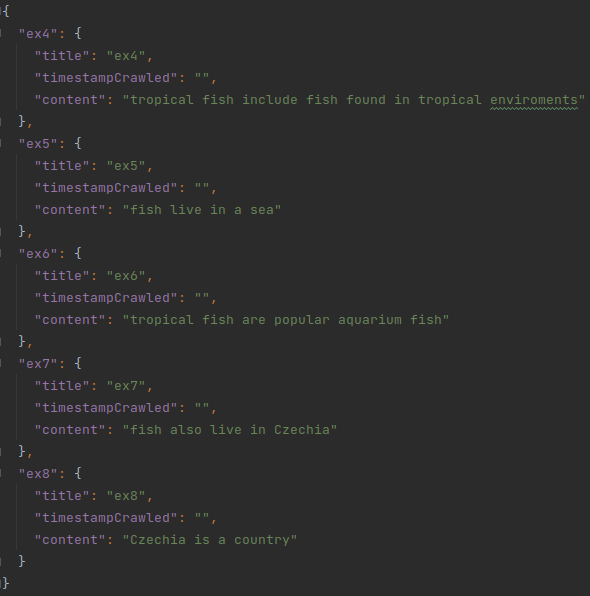
\includegraphics[width=\linewidth]{img/data}
    \caption{Data ze cvičení}
    \label{fig:data}
\end{figure}

\begin{figure}[H]
    \centering
    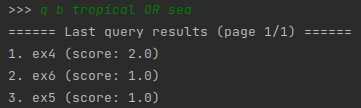
\includegraphics[width=\linewidth]{img/bool_one}
    \caption{Výsledek prvního dotazu}
    \label{fig:bool_one}
\end{figure}

\begin{table}[H]
    \begin{center}
        \begin{tabular}{ | m{0.5\textwidth} | m{0.5\textwidth} | }
            \hline
            Vytvoření indexu (přibližně z 10MB dat)
            & 30-40s \\
            \hline
            Vytvoření indexu (přibližně z 170MB dat)
            & 64\% po 2h - zrušeno \\
            \hline
            Kosinový dotaz nad tímto indexem (\uv{tropical fish sea}) - 121 výsledků
            & 3ms \\
            \hline
            Kosinový dotaz nad tímto indexem (\uv{magnum 357}) - 6333 výsledků
            & 35ms\\
            \hline
            Booleovský dotaz nad tímto indexem (\uv{tropical fish sea}) - 5 výsledků
            & 5ms \\
            \hline
            Booleovský dotaz nad tímto indexem (\uv{tropical OR fish OR sea}) - 121 výsledků
            & 1ms \\
            \hline
            Booleovský dotaz nad tímto indexem (\uv{magnum 357}) - 10 výsledků
            & 1ms \\
            \hline
            Booleovský dotaz nad tímto indexem (\uv{magnum OR 357}) - 6333 výsledků
            & 37ms\\
            \hline
        \end{tabular}
        \caption{Vlastní statistiky pro evaluaci systému}
        \label{table:statistics}
    \end{center}
\end{table}
%
%
\section{Závěr}
Tato práce demonstruje jednoduchý vyhledávací systém. Systém umožňuje za indexovat dokumenty a poté nad indexem
provádět dotazy. Indexy je do určité míry možné ovlivnit nastavením parametrů indexu. Indexy mohou být ukládány a
načítány ze souborů.

Práci je určitě možné vylepšit řadou funkcí a optimalizací. Na některých místech by bylo možné ušetřit operační
paměť lepším návrhem základní struktury indexu. Další dobré rozšíření by byl \uv{lazy loading} dokumentů, který
momentálně není implementován. Vhodnou optimalizací by bylo například zaměření se na snížení času indexace, protože
přibližně 10MB dat se indexuje zhruba 30 vteřin.
%%%
%%%
\end{document}
